
\section{Introduction}
Within systems neuroscience, significant efforts have been made to elucidate and analyze and the neural representation of objects and their categories. In humans, visual object recognition is generally accomplished rapidly and with minimal conscious effort, however this belies the true complexity of the task. And, while a practical mechanistic understanding of object recognition may currently fall beyond our reach, significant progress has been made in investigating the spatio-temporal dynamics of the process. 

Electroencephalography (EEG) has played an important role in these advances. Owing to its high temporal resolution, EEG allows us to investigate the rapid transformations of neural activity that underlie perception. In particular, EEG decoding studies have proven a popular paradigm in this area of research. In a decoding study, stimuli are presented to subjects, and contemporaneous neural responses to these stimuli are recorded. A decoding model is then trained on these responses to discriminate the property of interest. Frameworks such as representational similarity analysis (RSA) can be used to investigate organization of neural responses by comparing the similarity of patterns learned by a decoding model across conditions~\cite{Kriegeskorte:2008}. However, due to the complexity of the process, the noise inherent to the recording modality, and the resource intensive nature of data acquisition, EEG decoding presents substantial challenges.  

In this work, we attempt to replicate a target study which sought to extend this line of inquiry by introducing a novel classification-based RSA method~\cite{Kaneshiro:2015}. Rather than deriving representational dissimilarity matrices (RDMs) from pairwise classification accuracies, as done in prior work, the authors employed confusion matrices from multi-class classifiers applied to single-trial EEG data. This method was intended to determine whether emergent properties arising from the simultaneous consideration of multiple classes would yield a richer and more informative representational structure than traditional pairwise approaches. Additionally, the study aimed to localize the spatial and temporal components of EEG activity that contributed most strongly to category-level and exemplar-level distinctions. The reported findings appeared to support the effectiveness of this approach. In our replication attempt, we show that, while it is possible to replicate the primary results of the target study using an independent implementation of their analysis pipeline, the validity of these results is suspect. 

Recent work has demonstrated that the repetition of stimuli featured in the dataset collected by the target study introduces a methodological confound which substantially overestimates the separability of different object categories~\cite{Kilgallen:2025}. However, the extent to which this confound affects analyses performed in the target study has not yet been established. Our replication attempt is intended to assess this gap in the literature. Furthermore, a systematic review of the target study identified four additional limitations that undermine the validity of its findings

\begin{enumerate}[label=\Roman*]
    \item \label{enum:pc-leakage} The principal components of the entire feature matrix of each subject are used to reduce the dimensionality of the data, thereby ensuring that features of test data are leaked to training data.
    \item \label{enum:flawed-measure} The measure of dissimilarity used to perform representational similarity analysis is flawed as, in some cases, it results in negative values.
    \item \label{enum:outcome-dependence} The assessment of statistical significance is suspect as the study uses the binomial test to compare the number of correct predictions to chance level. However, each test set contains multiple responses to each stimulus, and consequently the assumption of independence between outcomes does not hold.
    \item \label{enum:multiple-comparisons} The validity of results deemed statistically significant by the target study is further undermined by the extensive number of hypothesis tests performed in the analysis of spatially and temporally resolved decoding experiments, given the absence of correction for the multiple comparisons incurred.
\end{enumerate}

Taken together, these limitations substantially undermine the evidential basis of the reported findings in the target study and necessitate appropriate mitigation to ensure the methodological robustness of our replication. 

\section{Materials and Methods}
\subsection{Data collection and processing in the target study}

The Stanford University Dataset (SUD) consists of preprocessed EEG recordings from 10 subjects, obtained while they viewed 72 images evenly distributed across 6 categories. To reduce the impact of trial-to-trial variation, each stimulus was presented 72 times to each subject, for a total of 5,184 trials per subject. The stimuli were recorded in six blocks of 864 trials each, over two sessions. In each block, all stimuli appeared 12 times, in a randomized order. Each stimulus was presented for 500~ms, followed by a 750~ms inter-stimulus interval, during which a gray background was displayed. The data was recorded using a 128-channel EEG system with a sampling rate of 1~kHz. The EEG signals were then preprocessed using a high-pass fourth-order Butterworth filter to attenuate frequencies below 1~Hz, and a low-pass Chebyshev Type I filter to attenuate frequencies above 25~Hz. The data was then subsampled to 62.5~Hz to reduce the computational cost of the analysis. Ocular artifacts were removed using the Bell-Sejnowski Infomax independent-component-analysis algorithm~\cite{Bell-Sejnowski:1995}.  The 4 channels used to detect ocular artifacts were removed, and the remaining channels were converted to average reference. Finally, epochs of 496~ms post-stimulus response, time-locked to the onset of the stimulus, were extracted from the data. As a result, each trial is represented as a 124$\times$32 feature matrix, where the first dimension represents the 124 channels which were retained, and the second dimension represents the 32 time points of post-stimulus response for each trial. See Fig.~\ref{fig:sud-category-structure} for a visualization of the category structure of the SUD. 

\begin{SCfigure}
    \centering
    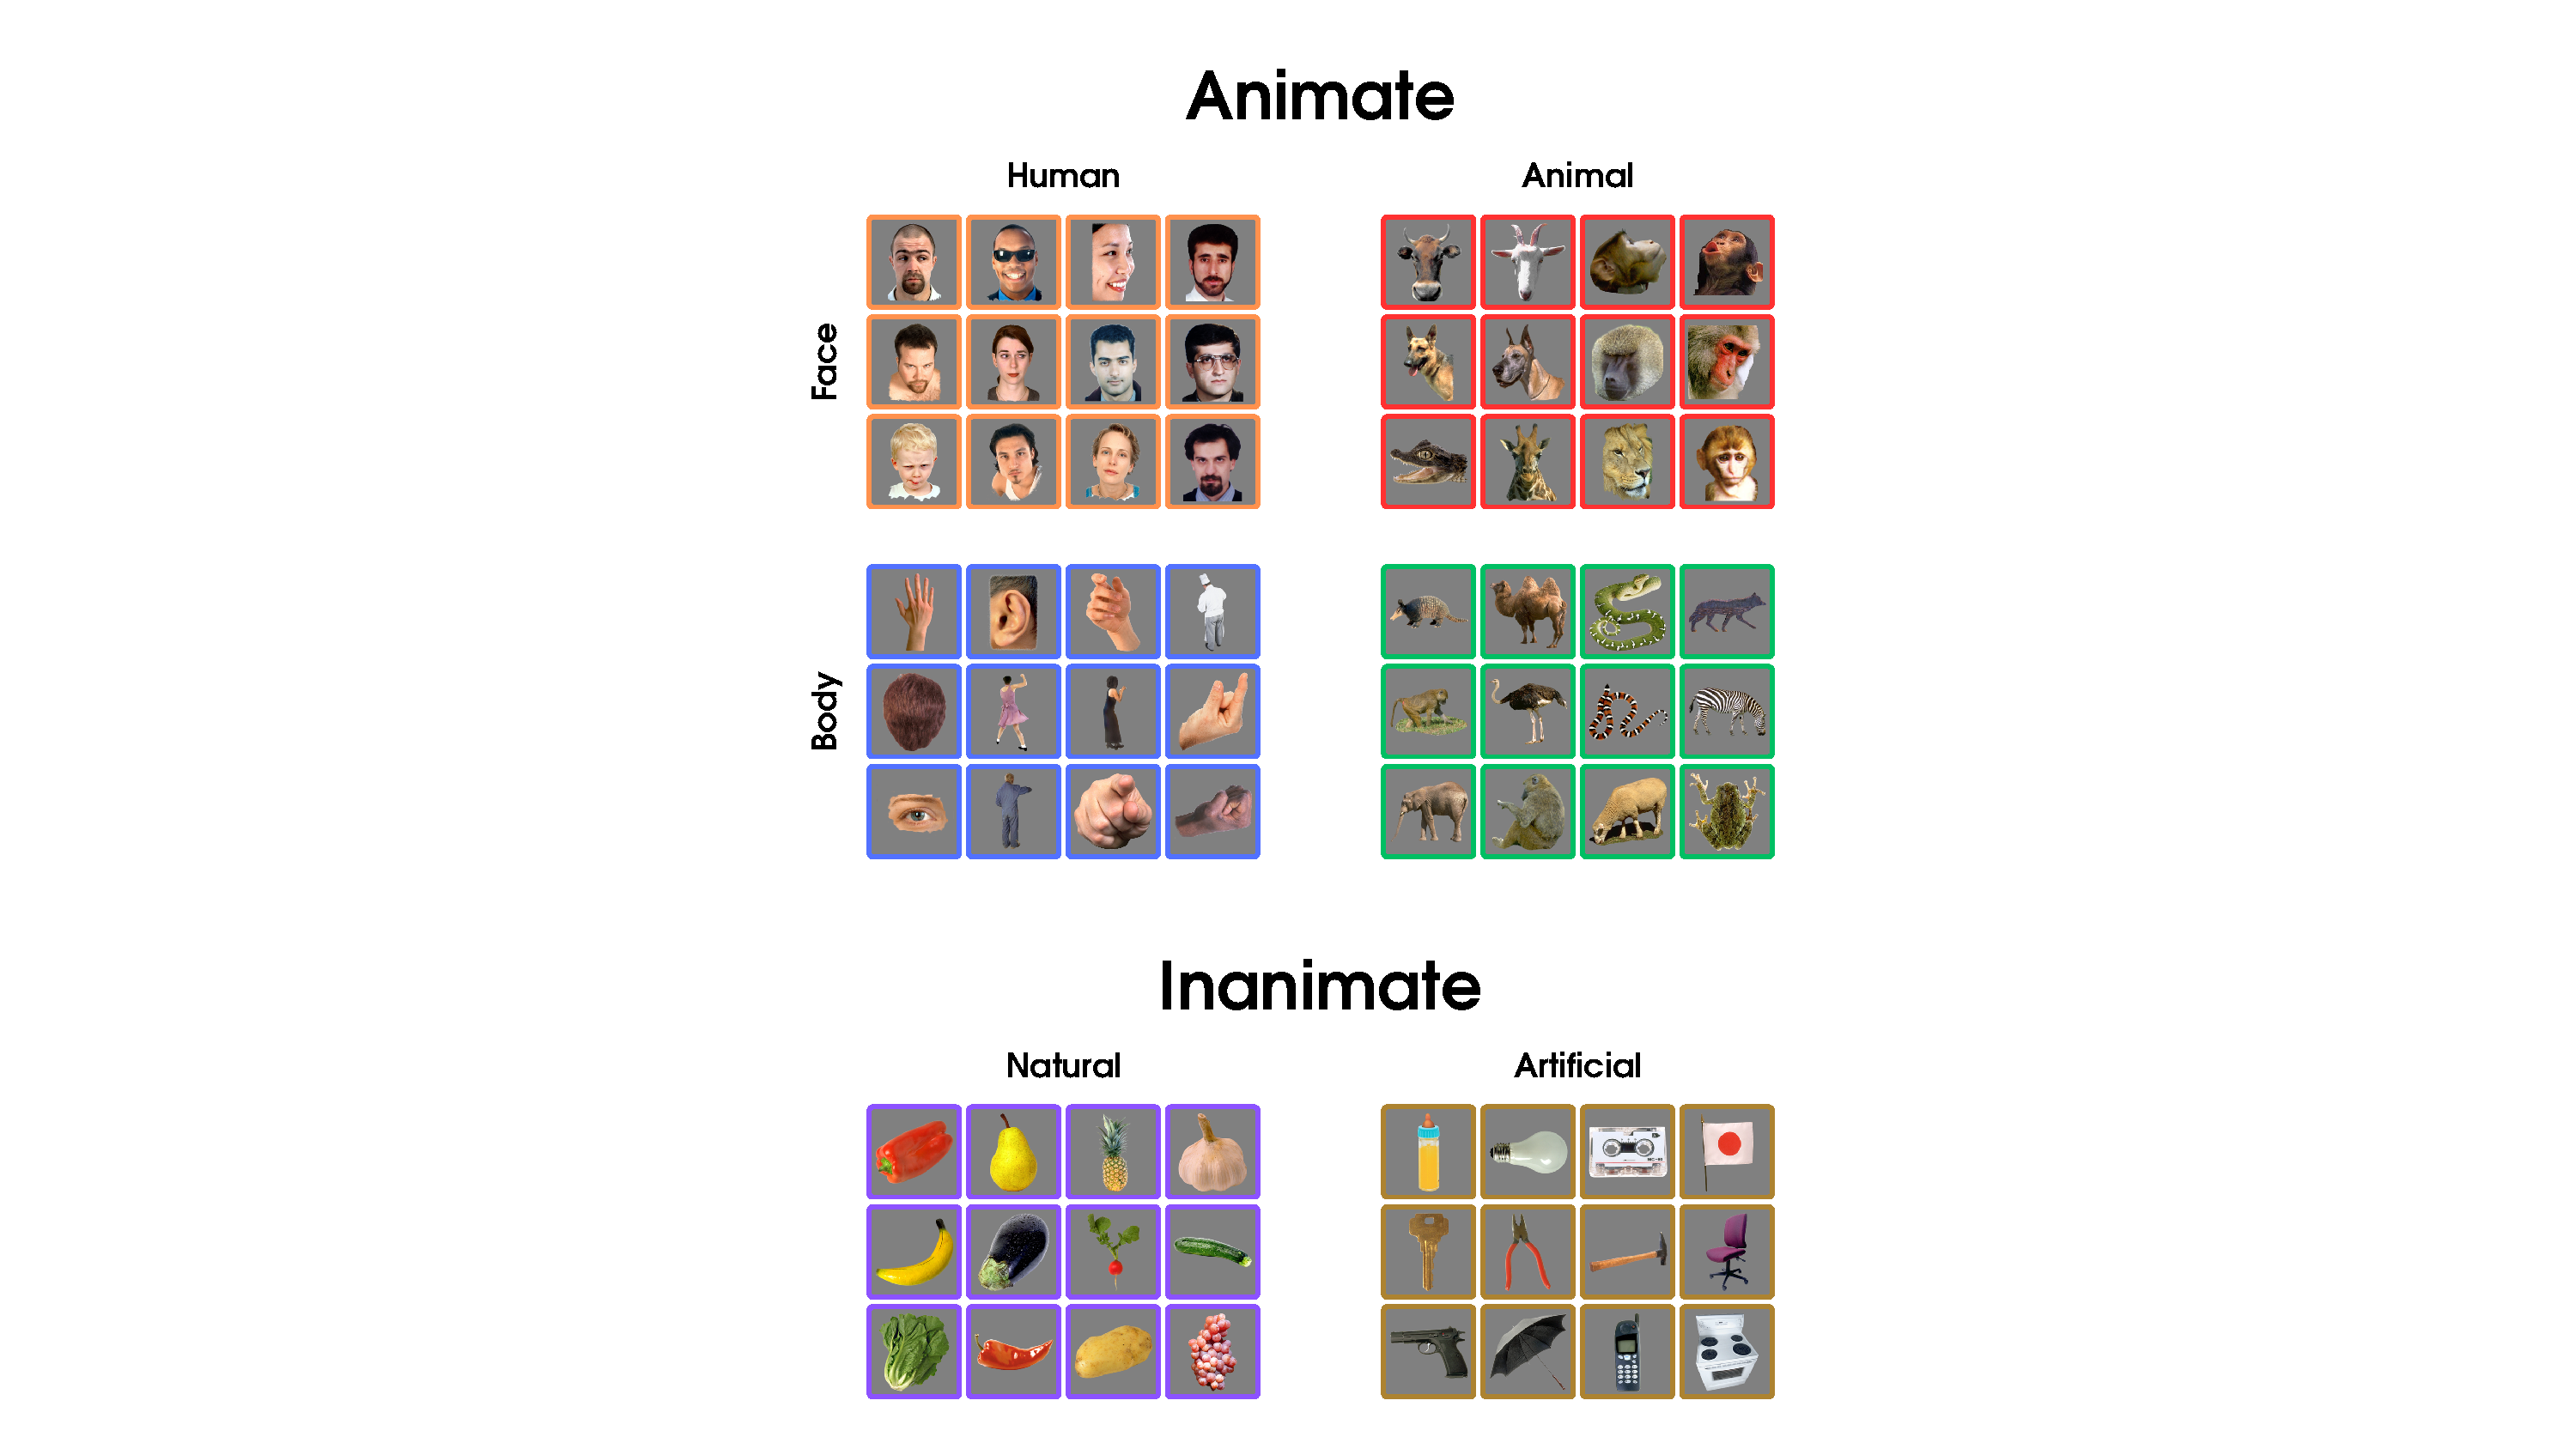
\includegraphics[width=7.5cm, trim={16cm, 0cm, 15cm, 1.0cm}, clip]{sudb_stimuli_by_category}
  \caption{\textbf{The category and structure of the SUD stimulus set.} The stimulus set used in the SUD is composed of 72 images of natural objects. These stimuli are evenly distributed across six categories: Human Body (HB), Human Face (HF), Animal Body (AB), Animal Face (AF), Fruit/Vegetable (FV), and Inanimate Object (IO). They additionally possess a coarse hierarchical structure using according to the Animate and Inanimate supercategories. Moreover,  the Animate category can be divided along two semantic : Human vs Animal, and Face vs Body. The colored borders framing each image are intended to clearly delineate object categories across visualizations and were not presented to subjects during the data collection process.\vspace{4.5em}}
  \label{fig:sud-category-structure}
\end{SCfigure}

\subsection{The analysis pipeline of the target study}

\subsubsection{Decoding tasks}
The primary decoding analyses of the target study are intended to comprise five decoding tasks: two at the category level (category decoding and human-face vs. artificial-object decoding) and three at the exemplar level (exemplar decoding, human-face decoding, and artificial-object decoding). Four variants of each task were performed to isolate the spatio-temporal dynamics of object recognition. In the baseline task, decoding models were trained and evaluated using signals from all electrodes across all timepoints. To isolate spatial contributions, models were trained to decode the signals of individual electrodes. Similarly, to isolate the separability of classes over time, another task was performed in which models were trained on windows of consecutive time points. Finally, to assess spatio-temporal variability, a fourth task was performed by training models on temporal windows from individual electrodes.

\subsubsection{Model training, selection and evaluation procedures}

In all decoding tasks, within-participant classification was performed using Linear Discriminant Analysis (LDA) using a one-versus-all classification strategy. To reduce the dimensionality of the data, Principal Component Analysis (PCA) was performed using singular-value decomposition (SVD). For all tasks, nested cross-validation was performed using 10 outer folds and 9 inner folds. The inner cross-validation folds were used to select the optimal number of principal components to use in dimensionality reduction over the range \([3, \min\left (200, K\right )]\), where \(K\) is the number of features used in the specific decoding task. To reduce the computational expense of the hyperparameter selection process, the SVD of the entire feature matrix was evaluated prior to constructing the cross-validation folds. A new model instance is trained using the combined data of the inner folds and the selected the number of principal components, before being evaluated on the outer fold. The model predictions are used to construct a confusion matrix, which summarizes the misclassification rates between all classes. 
 
\subsubsection{Representational similarity analysis}
In representational similarity analysis (RSA), a measure of the dissimilarity between different values of a target property is used to investigate the representational structure of that property~\citep{Kriegeskorte:2008}. In the target study, the confusion matrices obtained during cross-validation are used to measure the dissimilarity of classes in a given task using the function described in Eq.~\ref{eq:dissimilarity-measure}.

\begin{equation}
    D_{ij} = 1 - \sqrt{\frac{C_{ij}}{C_{jj}}\cdot \frac{C_{ji}}{C_{ii}}} \label{eq:dissimilarity-measure}
\end{equation}

The resulting dissimilarity measure is then used to visualize the representational space of the target property using multidimensional scaling (MDS). Moreover, to complement the hierarchical categories features in the stimulus featured in the target study, dendrograms are used to visualize the structure of the representational space using hierarchical clustering, via an unweighted pair grouping method with averaging (UPGMA). 

\subsection{Mitigating the limitations of the target study}
%As mentioned previously, the methodology employed by the target study strategy suffers from four major issues. First, as multiple responses to each stimulus were recorded, the test data consists of responses to stimuli already used to train models, which inflates estimates of model accuracy in the category decoding and human face vs artificial object decoding tasks. Secondly, by using the SVD of the entire feature matrix in dimensionality reduction, features of the test set may leak to the training set further inflating accuracy. Thirdly, the dissimilarity measure used does not satisfy the requirements of a dissimilarity measure. In particular, if a class is misclassified more often than it is correctly classified, then the measure returns negative values which are outside the defined range of a dissimilarity measure. 

As mentioned previously, the limitations of the analysis pipeline described in the target study severely undermine the evidential basis of the reported findings. As a result, we were required to modify several aspects of the original analysis pipeline to ensure the validity of the findings we present in our attempt at replication. 

\subsubsection{Addressing the repeated-stimulus confound}
The most substantial limitation of the target study is the low ratio of unique stimuli to repetitions in its decoding dataset. In alternative paradigms such as Event-Related Potential (ERP) analysis, the repetition of trials can be beneficial as it can improve the signal-to-noise ratio of the collected data. However, if the primary goal of a study is to investigate the dynamics of object recognition, and the representational structure of object categories, then the repetition of stimuli introduces a confound. Specifically, since any given stimulus which is presented to a subject will influence the resulting neural response, and determine the category label assigned to that response, stimulus identity confounds the relationship between response and category. When assessing the separability of object categories, it is necessary to validate the ability of the decoding model using unseen examples of those categories, otherwise the performance of a model may merely reflect its ability to memorize idiosyncratic features related to specific examples. 

Consequently, the separability of object categories reported using "category-level" classifications in the target study is confounded. However, it is possible to mitigate the confound for the category-level decoding tasks by ensuring that all decoding models are evaluated on responses to stimuli not seen during training. 

The "exemplar-level" classification tasks performed in the target study are similarly confounded as each exemplar of a category is represented by a single stimulus, and therefore the task captures the ability of a decoding model to decode specific stimuli rather than genuine exemplar-level generalization. Moreover, as exemplar identity and stimulus identity are equivalent in the design of the target study, it is impossible to mitigate the confound in the exemplar-level tasks. As a result, while we report the  results of these tasks in the supplementary material to examine the computational reproducibility of the target study, we omit these analyses from our findings. 


In the case of the category-level tasks (category decoding and human face vs artificial object decoding), we employed the nested paired cross-validation strategy from~\textcite{Kilgallen:2025}. Under this strategy, for each trained model, decoding accuracy is reported on two test sets: (i) a confounded test set consisting of responses to the same stimuli seen during training; and (ii) a \emph{deconfounded} test set composed of responses to novel stimuli. This procedure is particularly suited to our purposes as it allows use to investigate the extent to which the findings of the target study are contingent on the repeated-stimulus confound. We replicate the stimulus-level tasks of the target study using a stimulus-stratified nested cross-validation procedure. 

However, while the target study employs 10-fold cross validation, this cannot be used to achieve class-balanced cross-validation folds which mitigate the repeated stimulus confound; consequently, we apply 12-fold cross validation in all experiments to ensure the comparability of results across procedures. Similarly, while the target study optimizes the number of hyperparameters in each fold using 9 nested cross-validation folds, our procedure instead features 11 nested folds. Moreover, the cross-validation procedure we apply ensures that each test set is stratified by class label which ensures the performance estimates in each fold are not biased towards specific classes. 

\subsubsection{Rectifying the application of PCA and RSA}
To preclude the leakage of information from the test set, within each inner and outer fold we implement principal component analysis by deriving the SVD of the train data, which is then used to represent both the train data and the relevant held out set with respect to the principal component basis of the training data.

%However, to determine the computational reproducibility of the target study, we perform additional experiments using the original method of dimensionality reduction. 

To ensure the validity of the dissimilarity measure used during RSA while ensuring maximal fidelity to the target study, we amend the proposed transform by truncating negative values to 0 as described in Eq.~\ref{eq:corrected-dissimilarity-measure}.

\begin{equation} 
    D_{ij}^{\star} =
    \begin{cases}
        D_{ij} & \text{if \(D_{ij}\geq 0\)}\\
        0 & \text{otherwise}
    \end{cases}
    \label{eq:corrected-dissimilarity-measure}
\end{equation}

\subsubsection{Preventing spuriously significant results}
As the independence of outcomes required for a binomial test cannot be satisfied for test sets which feature stimulus repetition, we adopt an alternative procedure. In all hypothesis tests, we compute subject level classification accuracies, and apply a one-sample t-test to assess if the population mean is significantly greater than chance accuracy at the \(\alpha=0.05\) confidence level. 

Where we compare the significance of decoding performance across tasks, we apply the Bonferroni-Holm procedure to control the family-wise error rate~\citep{Holm:1979}. This ensures that the probability of a spuriously significant accuracy does not increase with the number of tests performed. However, in instances where we assess the significance of spatially or temporally resolved classifications, we instead apply the two-stage Benjamini-Yekutieli procedure to control the false discovery rate~\citep{Benjamini:2006}. This procedure ensures that the proportion of spuriously significant results does not increase with the number tests performed, while retaining good statistical power. A significant advantage of this procedure is that significance across different analyses is directly comparable. For example, although the number of hypothesis tests in the spatio-temporally resolved classifications is an order of magnitude greater than that required for spatially resolved classifications, topographical visualizations of significance are directly comparable.


To ensure robust statistical inference, in all analyses, the significance of classification accuracy was evaluated using one-sample t-tests applied to the classification accuracies obtained for each subject. Similarly, where multiple hypothesis tests are performed, we apply an appropriate method of multiple comparison correction, the details of which are reported in the results section.

\section{Results}
Table~\ref{tab:full-response-summary} presents the results of the full-response decoding experiments for each task. To confirm the consistency of our independent implementation of the analysis pipeline, and to assess the extent to which the findings of the target study are contingent on stimulus repetition, we report accuracy under two evaluation procedures. One which is affected by the repeated-stimulus confound, and, where possible, one which mitigates the confound. The significance of all values in the table were adjusted using the Bonferroni-Holm procedure.

\begin{table}
    \caption{Summary of full-response classification results.\label{tab:full-response-summary}}
    
\begin{tabular}{lSSSSS}
    \toprule
    & \textbf{Category} & \textbf{Exemplar\textsuperscript{\dag}} & \textbf{HF\textsuperscript{\dag}} & \textbf{IO\textsuperscript{\dag}} & \textbf{HF vs IO}\\
    & \textbf{(6 class)} & \textbf{(72 class)} & \textbf{(12 class)} & \textbf{(12 class)} & \textbf{(2 class)}\\    
    \midrule
    \multicolumn{6}{l}{\textbf{Deconfounded}}\\
    \quad Accuracy (\%) & 35.94\textsuperscript{***} & {---} & {---} & {---} & 79.82\textsuperscript{***}\\
    \quad SD & 5.00 & {---} & {---} & {---} & 3.70\\
    \quad Effect size & 3.86 & {---} & {---} & {---} & 8.06\\
    \multicolumn{6}{l}{\textbf{Confounded}}\\
    \quad Accuracy (\%) & 40.39\textsuperscript{***} & 11.68\textsuperscript{***} & 17.55\textsuperscript{***} & 30.68\textsuperscript{***} & 81.37\textsuperscript{***}\\
    \quad SD & 6.28 & 5.75 & 4.58 & 10.62 & 4.24\\
    \quad Effect size & 3.78 & 1.79 & 2.01 & 2.10 & 7.40\\ 
    % \multicolumn{6}{l}{\textbf{RSC + PCA leakage}}\\
    % \quad Accuracy (\%) & 40.39\textsuperscript{***} & 11.68\textsuperscript{***} & 17.55\textsuperscript{***} & 30.68\textsuperscript{***} & 81.37\textsuperscript{***}\\
    % \quad SD & 6.28 & 5.75 & 4.58 & 10.62 & 4.24\\
    % \quad Effect size & 3.78 & 1.79 & 2.01 & 2.10 & 7.40\\       
\bottomrule
\multicolumn{6}{p{0.9\linewidth}}{\small `\dag' indicates that the repeated-stimulus confound cannot be mitigated for the task.}\\
\multicolumn{6}{p{0.9\linewidth}}{\small `*', `**', and `***' indicates is greater than chance-level accuracy at the $p < 0.05$, $p < 0.01$, and $p < 0.001$ significance levels, respectively.}
\end{tabular}

        
\end{table}

The classification accuracies obtained under the repeated-stimulus confound we observe values comparable to those reported in the target study; 40.39\% vs 40.68\%, 11.68\% vs 14.46\%, 17.55\% vs 18.3\%, 30.68\% vs 28.87\% and 81.37 vs 81.08\% for the category, exemplar, human face, and human face vs artificial object decoding tasks respectively. This indicates that our independent implementation of the pipeline is a reasonable approximation of that employed in the target study. However, we emphasize that these results should not be construed as estimates of the separability of the classes in the corresponding tasks. Due to the equivalence of exemplar identity and stimulus identity under the design of the target study, it is impossible to mitigate the repeated-stimulus confound in the exemplar-level tasks. Consequently, while we report the full results of all experiments in the supplementary material; the remainder of our analyses are limited to the deconfounded category.

\subsection{The representational structure of object categories}
When the repeated-stimulus confound is mitigated, the classification accuracy for the 6 class full-response category decoding task drops from 40.39\% to 35.94\%. A paired t-test confirmed the significance of this discrepancy with confidence level \(\alpha=0.05\). This suggests that the repetition of stimuli in the target study results in a significant overestimation of the separability of categories. We observe a less discrepancy in performance on the human face vs artificial object decoding task (79.82\% vs 81.37\%). 

However, our findings differ from those reported in the target study beyond simple discrepancies in decoding accuracy. We present visualizations of the representational space formed by object categories in Fig.~\ref{fig:category-representation}. The multidimensional scaling plot shown in the target study suggested little separability between the human body and animal body categories. However, our results demonstrate that when the limitations of the target study are mitigated, all animate categories show significant separability. Similarly, the confusion matrix, multidimensional scaling plot, and dendrogram visualizing our results all suggest that the inanimate object categories are far less separable than was reported in the target study. Lastly, our results confirm that the human face category is classified successfully more than any other category as claimed in the target study. We omit the presentation of similar visualizations for the human face vs artificial object decoding task as binary classification results in a trivial representational space.

\begin{figure}
    \begin{minipage}[b]{0.32\columnwidth} 
        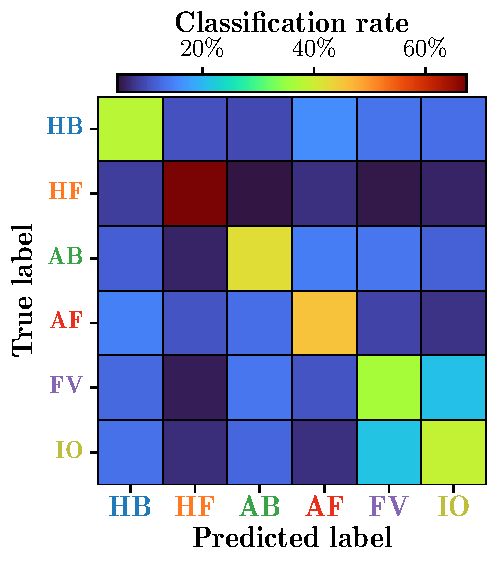
\includegraphics[width=\columnwidth]{SUDB_full_response_category_decoding/LDA/all_electrodes/all_timepoints/unconfounded_test/confusion_matrix}
    \end{minipage}
    \begin{minipage}[b]{0.32\columnwidth}
        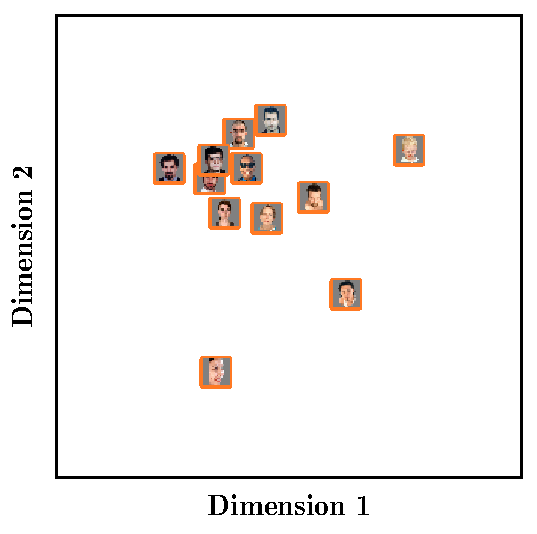
\includegraphics[width=\columnwidth]{SUDB_full_response_category_decoding/LDA/all_electrodes/all_timepoints/unconfounded_test/MDS}
    \end{minipage}
    \begin{minipage}[b]{0.32\columnwidth}
        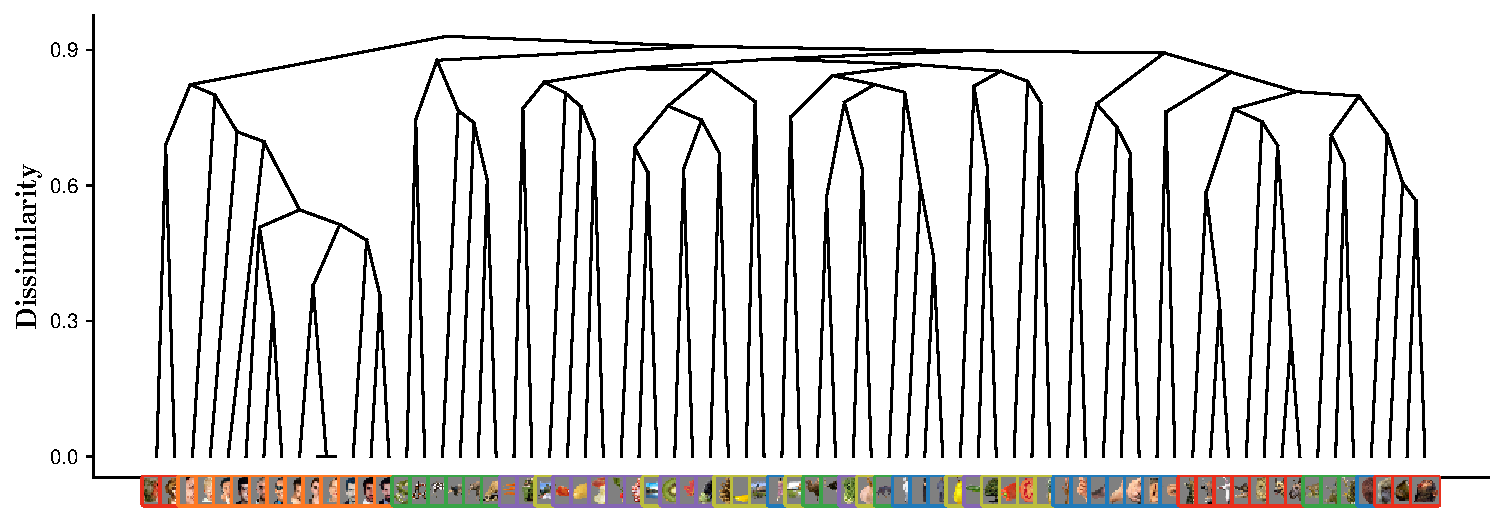
\includegraphics[width=\columnwidth]{SUDB_full_response_category_decoding/LDA/all_electrodes/all_timepoints/unconfounded_test/dendrogram.pdf}
    \end{minipage}
    \caption{\textbf{The representational structure of object categories is significantly misrepresented in the target study.} While the target study observed that the inanimate object categories exhibited the least separation, their findings still demonstrate robust dissimilarity between them. However, the dendrogram we derived suggests that the target study considered them to be more than twice as separable as they actually are. \label{fig:category-representation}}
\end{figure}


\subsection{The topography of object category separability}
To investigate the spatial distribution of category selectivity, we constructed topographic maps illustrating the distribution of category decoding accuracies for models trained on the signals of individual electrodes as seen in Fig.~\ref{fig:category-topomaps}. The statistical significance of the accuracy for each electrode was assessed using a one-sample t-test with confidence level \(\alpha=0.05\). The  Given the extent of the multiple comparisons incurred by assessing the separability of object categories for the signals recorded at each location, we apply the two-stage Benjamini-Yekutieli procedure to ensure the false discovery.

Our results suggest that the repeated-stimulus confound not only misrepresents of the representational space of object categories, but the spatial dynamics of object processing as well. In particular, we find that the separability of categorical information is disproportionately exaggerated for electrodes situation over the occipital cortex for both tasks. However, our findings also concur with the target study with respect to the general regions which exhibit the separability of categories. Moreover, the involvement of these observed regions is further corroborated by prior neuroimaging work~\cite{Itier:2004}.

\begin{figure}
    \centering
    \begin{minipage}{0.45\columnwidth} 
    \includegraphics[width=\columnwidth]{SUDB_single_electrode_category_decoding/LDA/all_timepoints/unconfounded_test/topomap.pdf}
    \subcaption{Category}    
    \end{minipage}
    \hfill
    \begin{minipage}{0.45\columnwidth} 
    \includegraphics[width=\columnwidth]{SUDB_single_electrode_human_face_vs_artificial_object_decoding/LDA/all_timepoints/unconfounded_test/topomap.pdf}
    \subcaption{HF vs IO}
    \end{minipage}  
    \caption{\textbf{The separability of object categories in the occipital cortex is exaggerated in the target study.} While the target study asserts that the right lateral region of the occipital cortex contains a cluster of electrodes which feature high levels of separability between object categories, out findings suggest that the relative performance of the region was significantly exaggerated. Given the central role of the occipital cortex in the early stages of visual processing, this finding may be explained by the memorization of low-level stimulus specific features under the repeated-stimulus confound.  
    \label{fig:category-topomaps}}
\end{figure}

\subsection{The temporal dynamics of object recognition}
In Table~\ref{tab:temporally-resolved} we report the results of the temporally resolved decoding analyses. The statistical significance of classification accuracies were assessed using a one-sample t-test with confidence level \(\alpha=0.05\). To account for the multiple comparisons across decoding tasks and temporal windows, the significance of results within each table are adjusted using the two-stage Benjamini-Yekutieli procedure to control the false discovery rate~\citep{Benjamini:2006}.

\begin{table}
    \caption{Summary of the temporally-resolved decoding analyses.\label{tab:temporally-resolved}}
    \resizebox{\textwidth}{!}{
\begin{tabular}{lSSSSSSSSS}
    \toprule
    & \textbf{0-80ms} & \textbf{48-128ms} & \textbf{96-176ms} & \textbf{144-224ms} & \textbf{192-272ms} & \textbf{240-320ms} & \textbf{288-368ms} & \textbf{336-416ms} & \textbf{384-464ms}\\
    \midrule
    
        \multicolumn{10}{l}{\textbf{Category}}\\
        \quad Accuracy (\%) & 16.79\textsuperscript{*} & 20.08\textsuperscript{***} & 30.69\textsuperscript{***} & 35.57\textsuperscript{***} & 35.11\textsuperscript{***} & 30.59\textsuperscript{***} & 26.89\textsuperscript{***} & 23.51\textsuperscript{***} & 23.03\textsuperscript{***}\\
        \quad SD & 0.67 & 1.82 & 4.16 & 5.00 & 4.34 & 3.04 & 2.77 & 2.42 & 2.79\\
        \quad Effect size & 0.18 & 1.88 & 3.37 & 3.78 & 4.25 & 4.59 & 3.69 & 2.82 & 2.28\\

	
        \multicolumn{10}{l}{\textbf{HF vs IO}}\\
        \quad Accuracy (\%) & 49.96\textsuperscript{} & 58.72\textsuperscript{***} & 75.32\textsuperscript{***} & 78.79\textsuperscript{***} & 75.55\textsuperscript{***} & 69.77\textsuperscript{***} & 62.46\textsuperscript{***} & 60.23\textsuperscript{***} & 61.73\textsuperscript{***}\\
        \quad SD & 1.48 & 3.82 & 4.66 & 5.33 & 3.38 & 4.47 & 5.64 & 5.77 & 4.92\\
        \quad Effect size & -0.03 & 2.28 & 5.43 & 5.40 & 7.56 & 4.42 & 2.21 & 1.77 & 2.38\\
         
\bottomrule
\multicolumn{10}{l}{\small `*', `**', and `***' indicates is greater than chance-level accuracy at the $p < 0.05$, $p < 0.01$, and $p < 0.001$ significance levels, respectively.}
\end{tabular}

}
        
\end{table}

We find that the separability of object categories is disproportionately overestimated in the target study over the 80--224~ms post-stimulus interval. This may be explained by a delay the recognition of object categories relative to the perception of their low-level features. Moreover, while we report approximately the same decoding accuracy as the target study over the 0--80~ms post-stimulus interval, our hypothesis tests contradict the claim that the observed accuracy is not statistically significant.

 However, our findings concur with the overall characterization of the temporal dynamics of object category-separability described in the target study. Specifically, our findings support the following claims made in the target study: (i) classification accuracy is near chance for all object categories over the 0--80~ms post-stimulus interval; (ii) separability of object categories is statistically significant for all subsequent temporal windows; (iii) peak decoding accuracy is achieved for the 144--224~ms post-stimulus temporal window; and (iv) decoding accuracy monotonically decreases over the subsequent temporal windows. See Fig.~\ref{fig:category-timecourse} for a visualization of the time-course of the classification accuracy by object category.

\begin{figure}
    \centering
    \begin{minipage}{\columnwidth} 
    \includegraphics[width=\columnwidth]{SUDB_temporal_window_category_decoding/LDA/all_electrodes/unconfounded_test/time_course.pdf}
    \subcaption{Category}
    \end{minipage}
    \hfill
    \begin{minipage}{\columnwidth} 
    \includegraphics[width=\columnwidth]{SUDB_temporal_window_human_face_vs_artificial_object_decoding/LDA/all_electrodes/unconfounded_test/time_course.pdf}  
    \subcaption{HF vs IO}      
    \end{minipage}
    \caption{\textbf{The separability of signals over temporally resolved classification windows.} In both decoding tasks, classification accuracy is approximately chance during the 0--80~ms response window. The temporal dynamics of classification accuracy are largely independent of object category. Generally, object category is most separable for the 144--224~ms response window, and subsequently monotonically increases. However, in both tasks, the separability of the human face category increases between the second last and last temporal windows. \label{fig:category-timecourse}}
\end{figure}

We find the temporal evolution of the representational structure of object categories is misrepresented in the target study. As in the full-response decoding analyses, the separability of the inanimate object categories is overestimated. Moreover, this overestimation is most prominent over the 80--224~ms post-stimulus interval, suggesting that meaningful distinctions between the neural representation of natural and artificial inanimate objects occur later in EEG data than suggested in the target study.

\begin{figure}
    \centering
    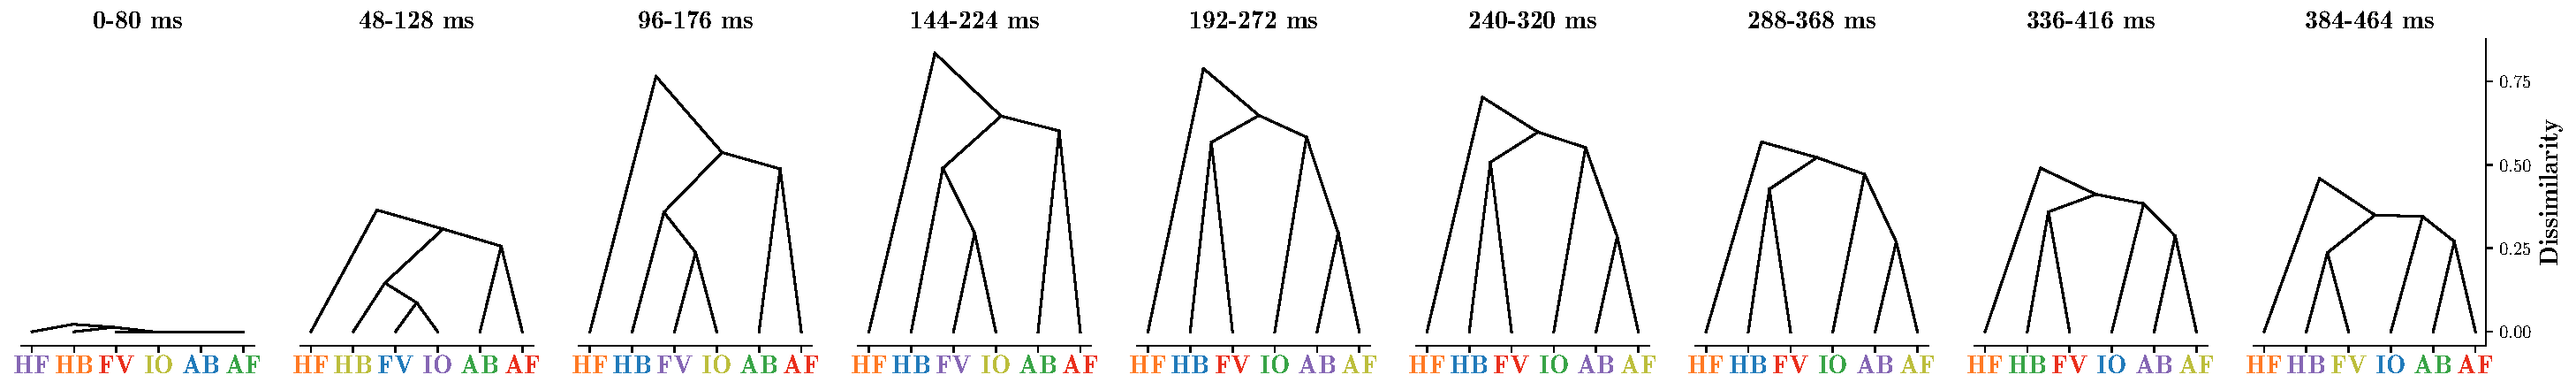
\includegraphics[width=\columnwidth]{SUDB_temporal_window_category_decoding/LDA/all_electrodes/unconfounded_test/dendrograms.pdf}        
    \caption{\textbf{The temporal evolution of object-category recognition.} While the evolution of the representational space is broadly similar when the confound is present (top) and when it is mitigated (bottom), we observe the same overestimation of separability in the inanimate object categories, particularly during the early temporal windows.\label{fig:category-temporal-dendrograms}}
\end{figure}

\subsection{The spatio-temporal dynamics of object-category recognition}
Lastly, the spatio-temporally resolved classifications conducted are visualized in Fig.~\ref{fig:category-spatiotemporal} using a sequence of topographical maps of classifier accuracy. To account for the multiple comparisons across electrodes and temporal windows, the significance of results within each table are adjusted using the two-stage Benjamini-Yekutieli procedure to control the false discovery rate.

\begin{figure}
    \centering
    \centering
    \begin{minipage}{\columnwidth} 
        \includegraphics[width=\columnwidth]{SUDB_single_electrode_temporal_window_category_decoding/LDA/unconfounded_test/topomaps.pdf}   
    \subcaption{Category}
    \end{minipage}
    \hfill
    \begin{minipage}{\columnwidth} 
        \includegraphics[width=\columnwidth]{SUDB_single_electrode_temporal_window_human_face_vs_artificial_object_decoding/LDA/unconfounded_test/topomaps.pdf}  
    \subcaption{HF vs IO}      
    \end{minipage}
    
          
    \caption{\textbf{Temporally resolved rate maps of the single-electrode decoding.} Our earlier finding that the repeated-stimulus confound exaggerates the relative separability of object categories for electrodes in the occipital region is also seen in the temporally resolved rate maps of both tasks. Moreover, our analysis suggests that the separability of object categories is not statistically significant during the 0--80ms post-stmulus interval as illustrated by the uncolored sections of the corresponding plots.\label{fig:category-spatiotemporal}}
\end{figure}


\section{Discussion}


\section{Conclusion}